% \begin{frame}
% 	\frametitle{Wirkungsquerschnitt}
% 	\begin{figure}
% 	\begin{center}
% 	  \includegraphics[width=0.3\textwidth]{../img/atlas_higgs_event.png}
% 	  \caption{Produkte einer Proton-Proton-Kollision beim ATLAS-Experiment am CERN (Quelle: https://cds.cern.ch/record/1459496)}
% 	\end{center}
% 	\end{figure}
% 	\begin{itemize}
% 		\item Bei Streuprozessen ist der Endzustand nicht eindeutig bestimmt
% 		\item Der Wahrscheinlichkeit eines bestimmten Endzustandes wird durch den Wirkungsquerschnitt $\sigma$ beschrieben.
% 		\item Differentieller Wirkungsquerschnitt $\frac{\difd \sigma}{\difd O}$ in Bezug auf \\
% 			  Observable $O$ (z.B. Raumwinkel $\Omega$, Transversalimpuls $p_\text{T}, \ldots$)
% 	\end{itemize}
% \end{frame}

\section{Theoretische Grundlagen}

\subsection{Das Standardmodell}
 \begin{frame}
 	\frametitle{Das Standardmodell}
 	\begin{figure}
 	\begin{center}
 	  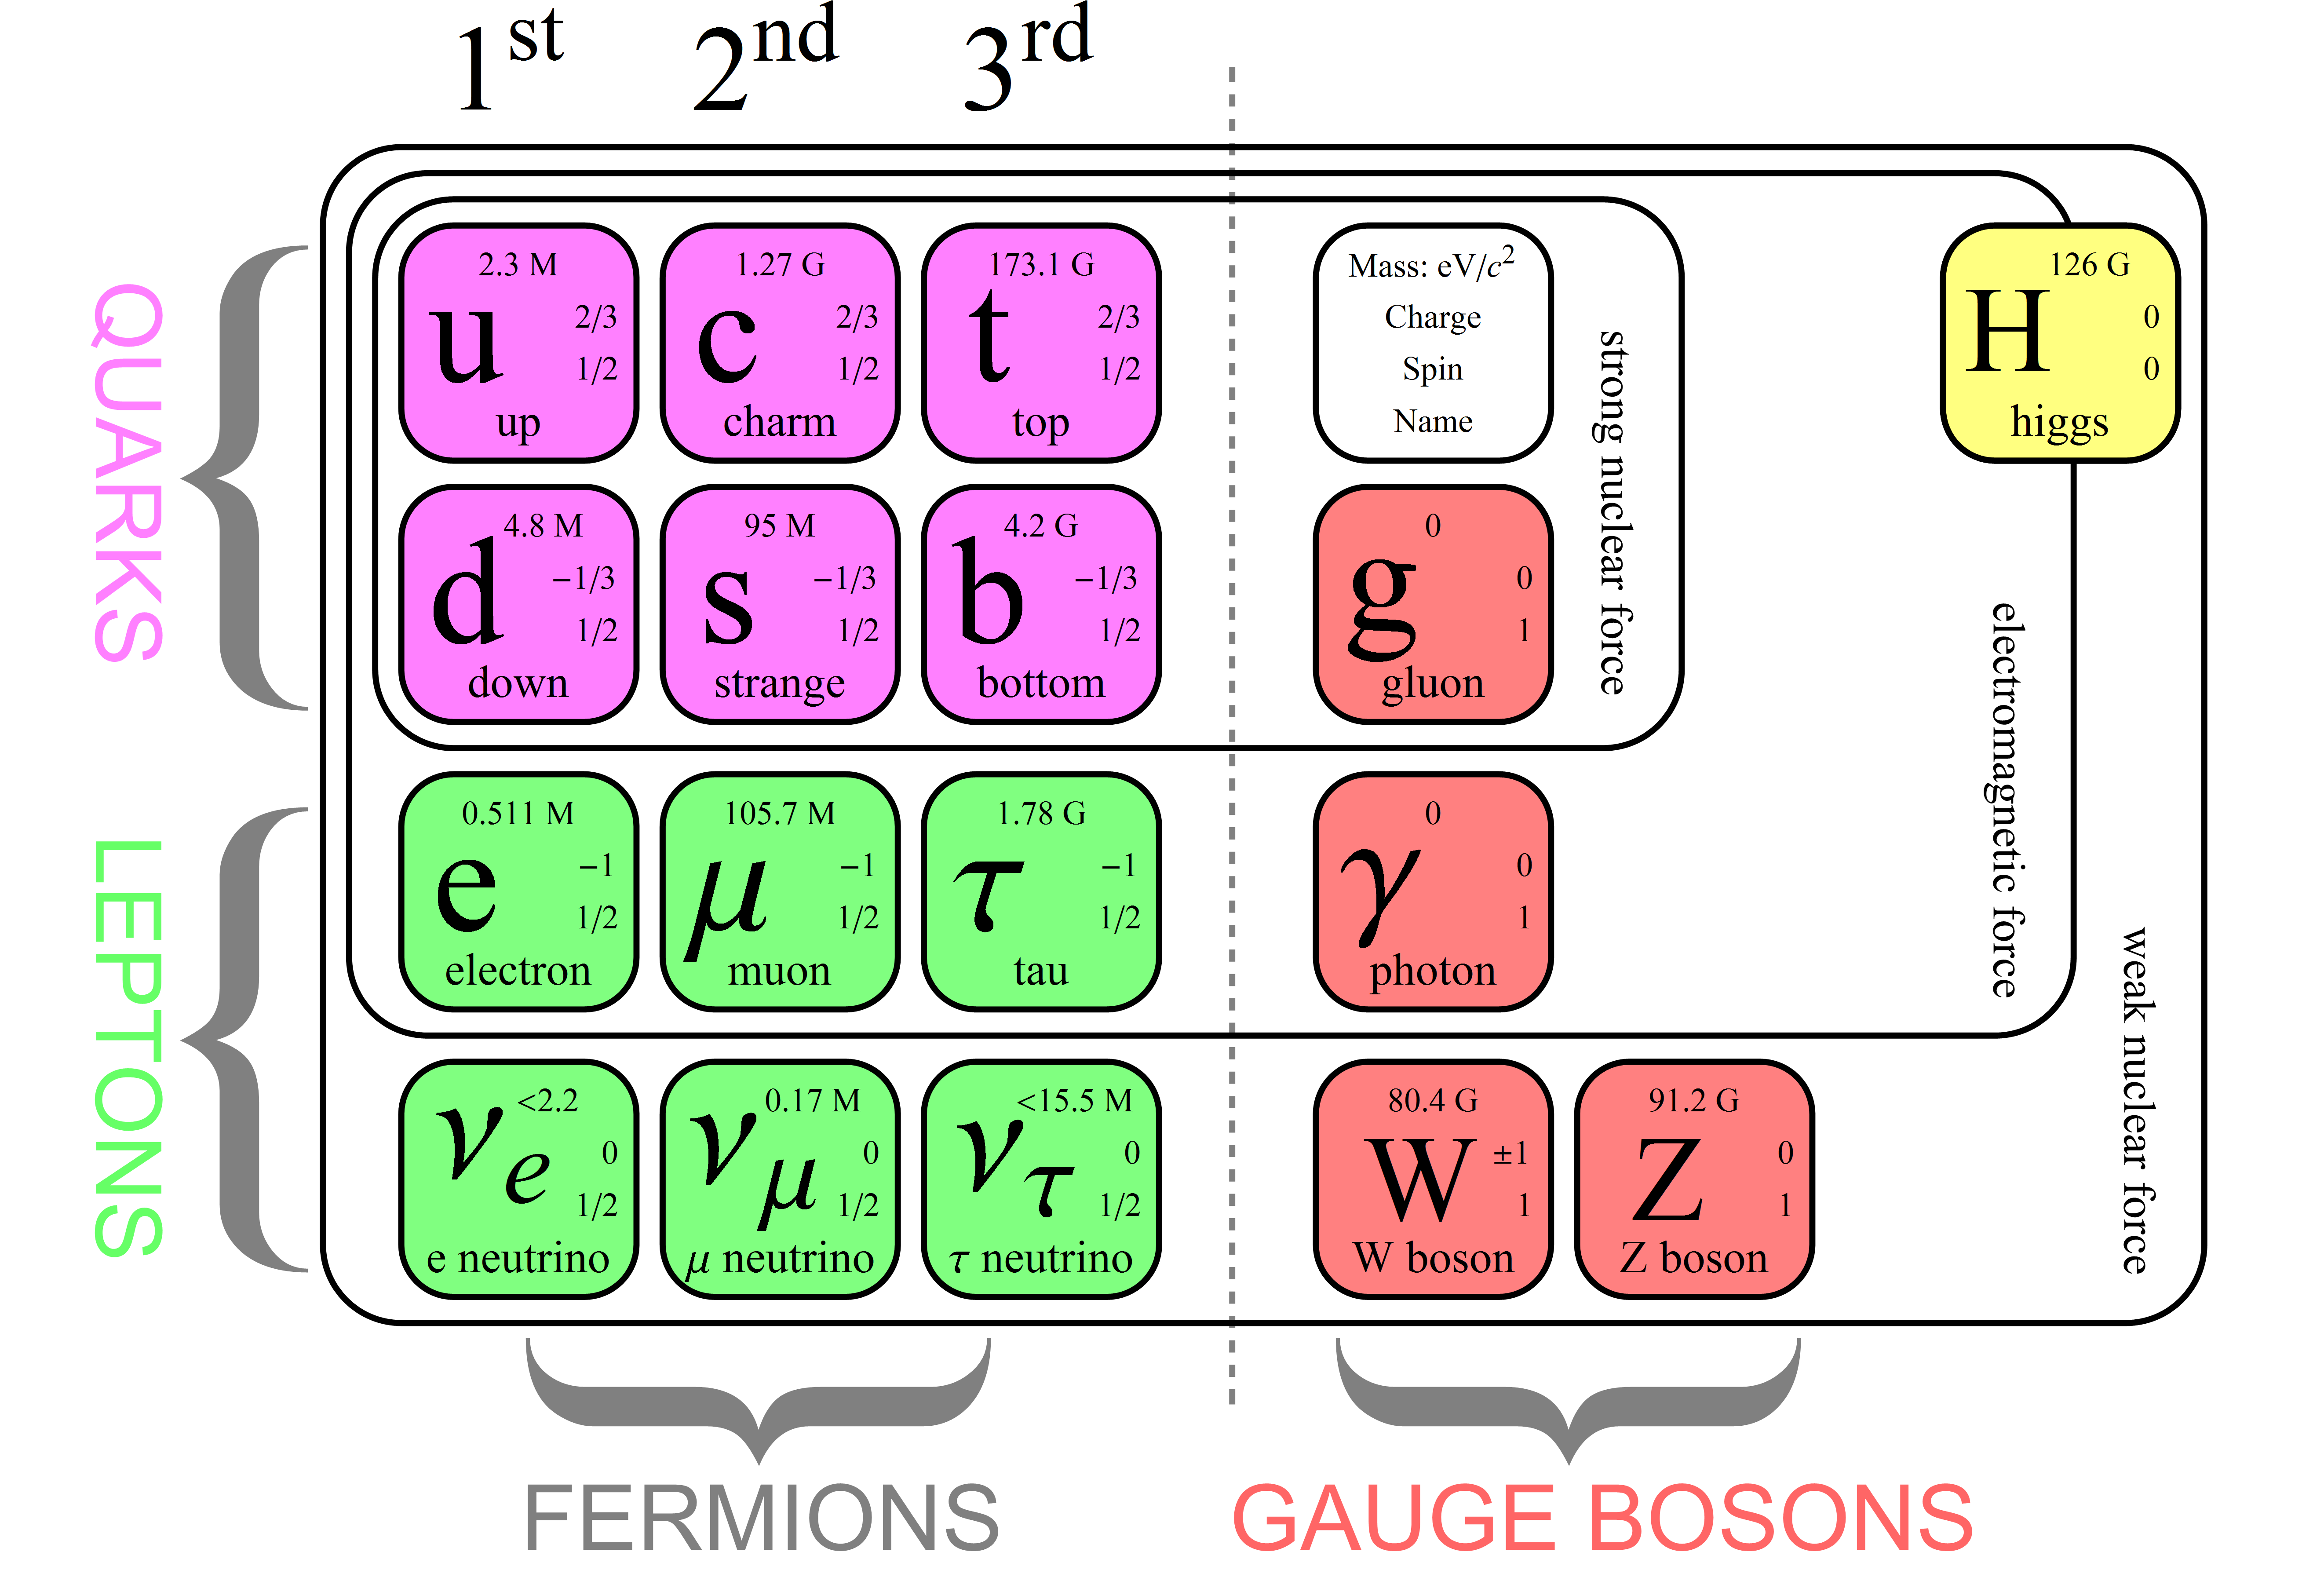
\includegraphics[width=0.66\textwidth]{graphics/SM1.png}
 	\end{center}
	\end{figure}
 \end{frame}
\subsection{Elektroschwache Wechselwirkung}
\begin{frame}
	\frametitle{Weinbergwinkel und Kopplungsstärken}
	\begin{center}
		\begin{equation*}
			\ket{\gamma} =  cos(\theta_w)\ket{B^0} + sin(\theta_w) \ket{W^0}
		\end{equation*}
		\begin{equation*}
		\ket{Z^0} = -sin(\theta_w) \ket{B^0} + cos(\theta_w) \ket{W^0}
		\end{equation}
	\end{center}
\end{frame}
\begin{frame}
	\frametitle{Weinbergwinkel und Kopplungsstärken}
	\begin{center}
		\begin{equation*}
		\ket{\gamma} =  cos(\theta_w)\ket{B^0} + sin(\theta_w) \ket{W^0}
		\end{equation*}
		\begin{equation*}
		\ket{Z^0} = -sin(\theta_w) \ket{B^0} + cos(\theta_w) \ket{W^0}
		\end{equation*}
		\begin{equation*}
			g_V^f = I^f_3-2 Q_f sin^2(\theta_w)
		\end{equation*}
		\begin{equation*}
			g_A^f = I^f_3
		\end{equation*}
	\end{center}
\end{frame}
\begin{frame}
	\frametitle{Vektor und Axialvektorkopplung}
	\begin{center}
	\end{center}
\end{frame}
\subsection{Wirkungsquerschnitt und Zerfallsbreite}

\subsection{$e^+e^-$ Kollisionen}
\begin{frame}
	\frametitle{Der Wirkungsquerschnitt}
	\begin{center}
		\begin{equation*}
		\sigma_f(s) = \frac{12\pi}{M_Z^2} \frac{s\Gamma_e\Gamma_f}{(s-M_Z^2)^2+s^2\Gamma_Z^2/M_Z^2}
		\end{equation*}
	\end{center}
\end{frame}

\subsection{Strahlungskorrektur}

\subsection{Vorwärts Rückwärts Asymmetrie}